\documentclass{article}


% if you need to pass options to natbib, use, e.g.:
%     \PassOptionsToPackage{numbers, compress}{natbib}
% before loading neurips_2023


% ready for submission
\usepackage{neurips_2023}


% to compile a preprint version, e.g., for submission to arXiv, add add the
% [preprint] option:
%     \usepackage[preprint]{neurips_2023}


% to compile a camera-ready version, add the [final] option, e.g.:
%     \usepackage[final]{neurips_2023}


% to avoid loading the natbib package, add option nonatbib:
%    \usepackage[nonatbib]{neurips_2023}


\usepackage[utf8]{inputenc} % allow utf-8 input
\usepackage[T1]{fontenc}    % use 8-bit T1 fonts
\usepackage{hyperref}       % hyperlinks
\usepackage{url}            % simple URL typesetting
\usepackage{booktabs}       % professional-quality tables
\usepackage{amsfonts}       % blackboard math symbols
\usepackage{nicefrac}       % compact symbols for 1/2, etc.
\usepackage{microtype}      % microtypography
\usepackage{xcolor}         % colors

\usepackage{verbatim}
\usepackage{stmaryrd}
\usepackage{tikz}
\usetikzlibrary{positioning, arrows.meta}
\usepackage{graphicx}
\usepackage{amsmath}
\usepackage{interval}


\title{Exploring the latent space of a temporal VAE for audio loops generation}


% The \author macro works with any number of authors. There are two commands
% used to separate the names and addresses of multiple authors: \And and \AND.
%
% Using \And between authors leaves it to LaTeX to determine where to break the
% lines. Using \AND forces a line break at that point. So, if LaTeX puts 3 of 4
% authors names on the first line, and the last on the second line, try using
% \AND instead of \And before the third author name.


%\author{AAAAA}

\date{}

\begin{document}


\maketitle
\vfill
\hspace*{-3cm}\rotatebox[origin=l]{90}{\vspace*{-10cm}\textcolor{gray}{\Huge\today}}\hspace*{1cm}


\begin{abstract}
    Generating diverse and high-quality audio samples is now possible thanks to deep generative models. As is the case for Variational Auto-Encoders [5], these models often rely on the generation of a low-dimensional latent space in which the characteristic information of the data is encoded. Decoding this space provides a trainable analysis-synthesis framework. We can then construct data, such as an audio signal, from a latent representation. The reconstruction will then have the same properties as the training data. So, this opens new horizons for artistic creation and for musical composition in particular. However, it is very tricky to represent the latent space to ourself and so to control it intuitively, especially since the latent variables are created without supervision. Our objective is then, based on the RAVE approach [1], to study a multimodal method in order to intuitively influence the latent space of the temporal Variational Auto-Encoder, pre-trained on electronic music loops.
    %, using a hand motion dataset. ??

\end{abstract}

% \begin{comment}
\section{Introduction}

Neural audio synthesis is nowadays an active research domain that opens new doors fo creativity, composition and sound design. Generating various high-quality audio samples is now possible thanks to generative models such as RAVE [1], which are capable of create new data which preserve the properties of the training data. To do so, deep generative approaches such as Variational Auto-Encoders [5] crate an low-dimensional latent space on which the data are encoded into latent variables. Decoding these then allows us to generate new data. However, the latent space is a theoretical consideration that is very complex to represent since the dimensions involved are still too big to understand. We therefore cannot exert an active and intuitive control over the latent space, nor evaluate the quality of such a space. Our goal will be then to explore and sample the latent space of a pre-trained VAE-based audio synthesis model in order to assess its quality and coverage. In the first place, we will look at the state-of-the-art data generation method. We will then train it on MNSIT in order to experiment and discuss qualitative results. Finally, we will dig into the Temporal Spectral VAE properly said.
%Latent space exploration ??

\section{State-of-the-art method}
%\label{gen_inst}

In this section, we shall emphasize the basic strategy we used to code our VAE. We will explain theoretically the VAE model and its loss, based on Kingma and Welling's article [5]. For this approach, we assume that the dataset is composed of $N$ i.i.d samples of a variable $x$ :

\begin{center}
    \[ x = \{x^{(i)}\}_{i=1,...,N}\]
\end{center}
We also assume that the data are generated by a random process, which involves a latent variable $z$. Let's assume that $z^{(i)}$ is generated by a prior distribution and $x^{(i)}$ by a conditional distribution as following :

\begin{center}
    \begin{align*}
        z^{(i)} &= p_{\theta^{*}}(z) \\
        x^{(i)} &= p_{\theta^{*}}(x | z),
    \end{align*}
\end{center}
with $p_{\theta^{*}}(z)$ and $p_{\theta^{*}}(x | z)$ belonging to a family of distribution $\{  ( \,p_{\theta^{*}}(z), \, p_{\theta^{*}}(x | z)\,) \,|\, \theta \in \Theta \}$. However, it is important to note that the parameter $\theta^*$ and all the latent variables are unknown ! The main issue will be to approximate them. The true posterior density is given by :
\begin{center}
    \[p_\theta(z | x).\]
\end{center}
Let us remember that
\begin{center}
    \[p_\theta(x|z) = \frac{p_\theta(x \cap z)}{p_\theta (z)}.\]
\end{center}

It follows that 

\begin{center}
        \[p_\theta(z)p_\theta(x|z) = p_\theta(x \cap z) = p_\theta(x)p_\theta(z|x),\]
\end{center}
and finally
\begin{center}
    \[ p_\theta(z|x) = \frac{p_\theta(x|z)p_\theta (z)}{p_\theta (x)}.\]
\end{center}
It is important to keep this equality in mind. However, the true posterior density $p_\theta(z|x)$ is intractable. Therefore, we must introduce a recognition model which will approximate this value. This how we define our encoder $q_\phi(z | x)$ : for a given datapoint $x$, $q_\phi$ produces variables from which $x$ could have been generated. Likewise, $p_\theta(x|z)$ is a probabilistic decoder : for a given latent variable $z$, it produces a distribution of possibly corresponding variables $x$. We will thus jointly optimize $\phi$ (the recognition model parameter) and $\theta$ (the generative model parameter). In order to do this, we will sum the log-likelihood over each datapoint : 
\begin{center}
    \[\log p_\theta(x^{(1)}, \ldots, x^{(N)}) = \sum_{i=1}^{N} \log p_\theta(x^{(i)}),\]
    
\end{center}

which can be rewritten as

\begin{center}
        \[\log p_\theta(x^{(i)}) = \mathcal{D}_{KL}(q_\phi(z | x^{(i)}) || p_\theta(z | x^{(i)})) + \mathcal{L}(\theta, \phi ; x^{(i)}), \quad \forall i \in \llbracket 1, N \rrbracket.\]
\end{center}

Since we want a high probability in this distribution of images, we shall maximize $\log p_\theta(x^{(i)})$. However, as we said above, the true posterior $p_\theta(z | x^{(i)})$ is unknown. We will therefore estimate $\log p_\theta(x^{(i)})$ by minimizing $\mathcal{D}_{KL}(q_\phi(z | x^{(i)}) || p_\theta(z | x^{(i)}))$ by $0$. Thus, we have, $\forall i \in \llbracket 1, N \rrbracket$:

\begin{center}

    \[\log p_\theta(x^{(i)}) \geq \mathcal{L}(\theta, \phi ; x^{(i)}) = \mathbb{E}_{q_\phi(z|x)} [- \log q_\phi(z|x) + \log p_\theta(x,z)],\]

\end{center}

which can be rewritten as


\begin{equation}\label{loss1}
    \mathcal{L}(\theta, \phi ; x^{(i)}) = -\mathcal{D}_{KL}(q_\phi(z | x^{(i)}) || p_\theta(z)) + \mathbb{E}_{q_\phi(z | x^{(i)})} [\log p_\theta(x^{(i)} | z)]
\end{equation}

%on a (\ref{loss1})

This will be our loss function. Note that the two terms correspond to two different losses :

\begin{equation*}
    \mathbb{E}_{q_\phi(z | x^{(i)})} [\log p_\theta(x^{(i)} | z)] :\ \texttt{reconstruction loss}\\
    \mathcal{D}_{KL}(q_\phi(z | x^{(i)}) || p_\theta(z)) :\ \texttt{regularization loss}.
\end{equation*}

The reconstruction loss increases the likelihood of the data generated given a configuration of the latent, while the regularization loss measures the proximity of the true prior $p_\theta (z)$ compared to the approximated posterior $q_\phi(z|x)$. This one allows the algorithm to optimize the choice of $q$ with respect to the true posterior distribution. 

Note that we sometimes prefer to use an extra parameter $\beta$ in order to adjust the weight of the regularization loss, as explained by Higgins et al [4] :

\begin{center}
    \begin{equation}\label{loss1beta}
        \mathcal{L}(\theta, \phi ; x^{(i)}) = - \beta \, \mathcal{D}_{KL}(q_\phi(z | x^{(i)}) || p_\theta(z)) + \mathbb{E}_{q_\phi(z | x^{(i)})} [\log p_\theta(x^{(i)} | z)].
    \end{equation}
\end{center}

We now want to optimize, thus differentiate, $\mathcal{L}(\theta, \phi; x^{(i)})$ with respect to $\theta$ and $\phi$. However, the differential of this loss in $\phi$ is poorly defined, and we need to reparametrize our problem.

In order to do that, we shall now introduce a little more complex sample generation method. Let us remeber that $z$ follows a conditional distribution $q_\phi (z | x)$. We will then express z as a deterministic variable $z=g_\phi (\epsilon, x)$ where $g_\phi$ is a parametric function of $\phi$ and $\epsilon$ is an auxiliary variable (a noise separately generated, usually Gaussian). 

In the case of our Variatioanal Auto-Encoder, we will assume that the prior $p_\theta (z)$ is a centered isotropic multivariate Gaussian $\mathcal{N}(z;0,I)$. Let the posterior $p_\phi (x | z)$ be a multivariate Gaussian or a Bernoulli. We will then assume that the approximated posterior $q_\phi (z|x)$ is a multivariate Gaussian such that


\begin{center}
    \begin{equation*}
        \log q_\phi(z|x^{(i)}) = \log \mathcal{N} (z; \mu^{(i)}, \sigma^{2(i)I})  
    \end{equation*}
\end{center}


where $\mu^{(i)}$ and $\sigma^{(i)}$ are the outputs of our encoder (non linear functions of $x^{(i)}$ and $\phi$). It can be showed that the good reparametrisation of our problem us given by :

\begin{center}
    \begin{equation*}
        z^{(i,l)} \sim q_\phi (z|x^{(i)})
    \end{equation*}
\end{center}
with 

\begin{center}
    \begin{equation*}
        z^{(i,l)} = g_\phi (x^{(i)}, \epsilon^{(l)}) = \mu^{(i)} + \sigma^{(i)}  \odot\epsilon^{(l)}
\end{equation*}
\end{center}
where 
\begin{equation*}
    \epsilon \sim \mathcal{N}(0,I)
\end{equation*}
and $\odot$ designates an element-wise product.

Since the prior and the approximated posterior are both Gaussians, it can be showed that the loss in (\ref{loss1}) can be brought back to :
\begin{equation}\label{loss2}
    \mathcal{L}(\theta, \phi; x^{(i)}) \approx \frac{1}{2} \sum_{j=1}^{J} (1 \,+\, \log((\sigma_j^{(i)})^2 \,-\, (\mu_j^{(i)})^2 \,-\,(\sigma_j^{(i)})^2)\,\,+\,\,\frac{1}{L}\sum_{l=1}^{L} \log p_\theta(x^{(i)} | z^{(i,l)})
\end{equation}
with
\begin{equation*}
    z^{(i,l)}=\mu^{(i)} + \sigma^{(i)} \odot \epsilon^{(l)}
\end{equation*}
and 
\begin{equation*}
    \epsilon^{(l)} \sim \mathcal{N}(0,I).
\end{equation*}


\begin{figure}[h]
    \centering
    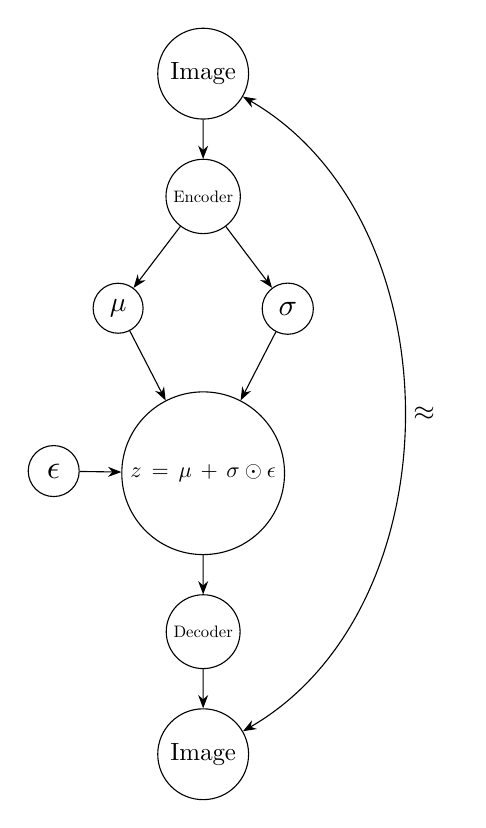
\begin{tikzpicture}[>=Stealth, node distance=0.5cm, scale=0.7]

        % Noeuds (cercles)
        \node [draw, circle, scale=0.9] (A) {Image};
        \node [draw, circle, below=of A, scale=0.6] (B) {Encoder};
        \node [draw, circle, below right=of B, xshift=-2cm, yshift=-0.5cm, scale=1] (C) {$\mu$};
        \node [draw, circle, below left=of B, xshift=2cm, yshift=-0.5cm, scale=1.1] (D) {$\sigma$};
        \node [draw, circle, below=of B, yshift=-1.5cm, scale=0.8] (E) {$z\,=\,\mu\,+\,\sigma \odot \epsilon$};
        \node [draw, circle, below left=of C, xshift=0cm, yshift=-1.25cm, scale=1.2] (eps) {$\epsilon$};
        \node [draw, circle, below=of E, scale=0.6] (F) {Decoder};
        \node [draw, circle, below=of F, scale=0.9] (G) {Image};

        % Flèches verticales
        \draw [->] (A) -- (B);
        \draw [->] (B) -- (C);
        \draw [->] (B) -- (D);
        \draw [->] (C) -- (E);
        \draw [->] (D) -- (E);
        \draw [->] (E) -- (F);
        \draw [->] (F) -- (G);
        \draw [->] (eps) -- (E);

        % Flèche courbée de A à G avec un angle plus important
        \draw [<->, bend left=60] (A) to node[midway, right] {$\approx$} (G);

    \end{tikzpicture}
    \caption{Complete diagram of the VAE with reparametrization}
    \label{VAE}
\end{figure}

\newpage


\section{Experiments on MNIST}
%\label{headings}


\section{Temporal Spectral VAE}

\section{Realtime Audio Variational autoEncoder (RAVE)}

In order to highlight the characteristic information of the latent space, we can adapt the Realtime Audio Variational autoEncoder method [1]. So, let us dig into the general procedure of this algorithm. 

When we code a VAE, the representation learned theoretically contains high-level features of the dataset. However, as we now want to deal with audio signals, we should consider a 
finer representation. Indeed, two similar signals can have slightly varying phases and result in totally different waveforms. Therefore, the reconstruction loss $\mathbb{E}_{q_\phi(z | x^{(i)})} [\log p_\theta(x^{(i)} | z)]$ 
described above, if calculated from the raw waveform, penalizes the learned model because the phase variations are not included in the representation. This can corrupt the training process and induce low-level variations of the audio signal in the latent space, which are not relevant for sound rendering. To fix this, we can split the training processus into two steps : representation learning and the adversarial fine-tuning.

So, the first step of the procedure is the representation learning. We will use the multiscale spectral distance $S$ described by Engel et al. [3] in order to estimate the distance between the synthetized and real waveforms, denifned by : 

\begin{equation} \label{spectral_dist}
    S(x,y) = \sum_{n \in \mathcal{N}}\, (\, \frac{\lVert STFT_n(x) - STFT_n(y) \rVert_F}{\lVert STFT_n(x) \rVert_F} \,+\, \log (\lVert STFT_n(x) - STFT_n(y) \rVert_1)   \,),
\end{equation}

where $\mathcal{N}$ designates the set of scales, $STFT_n$ the amplitude of the short term Fourier transform with a window size n and hop size n/4, $\lVert \,.\, \rVert_F$ the Frobenius norm and $\lVert \,.\, \rVert_1$ the $l^1$ norm. We will therfore use an amplitude spectrum-based distance, which will take into account the phase reconstruction errors and contain the caracteristic information of the signal.
We train the encoder and the decoder with the following loss :

\begin{equation}
    \mathcal{L}_{vae} (x) \,=\, \mathbb{E}_{\hat{x} \sim p(x|z)}(S(x,\hat x)) \,+\, \beta . \mathcal{D}_{KL}(q_\phi (z|x)||p(z)).
\end{equation}

We train the model with this loss and once it converges, we move on to the next step.

The second step aims to improve the audio quality and its natural appearance. Once we assume that the learned representation reached a satisfactory state, we only train the decoder using an adversarial objective. The GANs are an implicit generative model which allows to sample from a complex distribution by changing it in a simplier one, called base distribution. We use here the latent space learned in the first step as base distribution and we train the decoder to produce synthetised signals similar to real signals, using a discriminator D. We use the hinge loss version of the GAN objective, defined as :



\begin{align}
    \mathcal{L}_{dis}(x,z) &= \max(0, 1 - D(x)) + \mathbb{E}_{\hat x \sim p(x|z)}(\max(0, 1 + D(\hat x))) \\
    \mathcal{L}_{gen}(z) &= -\mathbb{E}_{\hat x \sim p(x|z)}(D(\hat x))
\end{align}

Since we do not want the synthetised signal $\hat x$ to diverge too much from the real signal $x$, we keep minimizing the spectral distance defined above (\ref{spectral_dist}) by adding the feature matching loss $\mathcal{L}_{FM}$ [6]. By combining everything, we end up at the wanted decoder :

\begin{equation}
    \mathcal{L}_{total} (x,z) \,=\, \mathcal{L}_{gen}(z)\,+\,\mathbb{E}_{\hat x \sim p(x|z)}(S(x, \hat x ) + \mathcal{L}_{FM}(x, \hat x)).
\end{equation}



Moreover, the loss we used in the first step consists of two terms : the  reconstruction term $\mathbb{E}_{\hat{x} \sim p(x|z)}(S(x,\hat x))$ and the regularisation term $\mathcal{D}_{KL}(q_\phi (z|x)||p(z))$. The reconstruction aims to maximise the mutual information between the latent representation and the data distribution while the regularisation tends to make the posterior distribution independent from data. The final objective guides the model to acquire condensed representations of the data. In this process, meaningful latent factors exhibit the greatest KL divergence from the prior distribution, whereas less informative latent factors have a KL divergence approaching zero, as outlined by Higgins et al. [4].

In order to better understand the latent representation, we will try to identify the most informative part of it. Our goal is to reduce the dimension of the representation learned to the minimum requierd to reconstruct the signal. To do this, we adapt the method for range and null space estimation to this problem.

Let $Z \in \mathbb{R}^{b \times d}$ a matrix composed of $b$ samples $z \in \mathbb{R}^d$, where $z \sim q_\phi(z|x)$. Since the collapsed parts of Z has a high variance, we first start to subtract the variance from Z by considering the matrix $Z' \in \mathbb{R}^{b \times d}$ :
\begin{equation}
    Z_i' = \text{argmax}_{z} q_\phi (z|x).
\end{equation}
Thus, the dimensions of the posterior distribution \(q_{\phi}(z|x)\) that have collapsed to the prior \(p(z)\) will yield a constant value in \(Z'\). To address this, we nullify this constant value by subtracting the mean of \(Z'\) along the first dimension. The only dimension of $Z'$ with values different from zero will be correlated to the input, which contais the informative part of the latent space.

We can now decompose this centerd matrix into singular values :
\begin{equation}
    Z'\,=\, U\, \Sigma \,^tV,
\end{equation}

where $\Sigma$ is composed by the singular values of $Z'$.
Then, it can be showed that the rank $r$ of $Z'$ is equal to the number of non-zero singular values of $Z'$ present in $\Sigma$. But the singular values that we want to identify as zero are not very likely to be strictly equal to zero, given the high variabilities in real data. So, if we want to find the rank of $Z'$, we must define a fidelity parameter $f \in [0,1]$ and the associated rank $r_f$ defined as the the smallest integer verifying :
\begin{equation}
    \frac{\sum_{i \leq r_f} \Sigma_{ii}}{\sum_i \Sigma_{ii}} \geq f.
\end{equation}

for a specific value of $f$ and a latent representation $z \sim q_\phi (z|x)$, we can reduce the dimension of $z$ by projecting it on the base defined by $^tV$. We then only keep the $r_f$ first dimensions to obtain a low-rank representation of $z_f$. Note that this dimension depends on $f$ and the dataset. Finally, we concatenate $z_f$ with a noise sampled from the prior distribution, we reproject it on the the original basis using $V$ and we give it to the decoder.

%\section{Citations, figures, tables}
%\label{others}
% \end{comment}
\begin{comment}
    

    These instructions apply to everyone.
    
    
    \subsection{Citations within the text}
    
    
    The \verb+natbib+ package will be loaded for you by default.  Citations may be
    author/year or numeric, as long as you maintain internal consistency.  As to the
    format of the references themselves, any style is acceptable as long as it is
    used consistently.
    
    
    The documentation for \verb+natbib+ may be found at
    \begin{center}
      \url{http://mirrors.ctan.org/macros/latex/contrib/natbib/natnotes.pdf}
    \end{center}
    Of note is the command \verb+\citet+, which produces citations appropriate for
    use in inline text.  For example,
    \begin{verbatim}
       \citet{hasselmo} investigated\dots
    \end{verbatim}
    produces
    \begin{quote}
      Hasselmo, et al.\ (1995) investigated\dots
    \end{quote}
    
    
    If you wish to load the \verb+natbib+ package with options, you may add the
    following before loading the \verb+neurips_2023+ package:
    \begin{verbatim}
       \PassOptionsToPackage{options}{natbib}
    \end{verbatim}
    
    
    If \verb+natbib+ clashes with another package you load, you can add the optional
    argument \verb+nonatbib+ when loading the style file:
    \begin{verbatim}
       \usepackage[nonatbib]{neurips_2023}
    \end{verbatim}
    
    
    As submission is double blind, refer to your own published work in the third
    person. That is, use ``In the previous work of Jones et al.\ [4],'' not ``In our
    previous work [4].'' If you cite your other papers that are not widely available
    (e.g., a journal paper under review), use anonymous author names in the
    citation, e.g., an author of the form ``A.\ Anonymous'' and include a copy of the anonymized paper in the supplementary material.
    
    
    \subsection{Footnotes}
    
    
    Footnotes should be used sparingly.  If you do require a footnote, indicate
    footnotes with a number\footnote{Sample of the first footnote.} in the
    text. Place the footnotes at the bottom of the page on which they appear.
    Precede the footnote with a horizontal rule of 2~inches (12~picas).
    
    
    Note that footnotes are properly typeset \emph{after} punctuation
    marks.\footnote{As in this example.}
    
    
    \subsection{Figures}
    
    
    \begin{figure}
      \centering
      \fbox{\rule[-.5cm]{0cm}{4cm} \rule[-.5cm]{4cm}{0cm}}
      \caption{Sample figure caption.}
    \end{figure}
    
    
    All artwork must be neat, clean, and legible. Lines should be dark enough for
    purposes of reproduction. The figure number and caption always appear after the
    figure. Place one line space before the figure caption and one line space after
    the figure. The figure caption should be lower case (except for first word and
    proper nouns); figures are numbered consecutively.
    
    
    You may use color figures.  However, it is best for the figure captions and the
    paper body to be legible if the paper is printed in either black/white or in
    color.
    
    
    \subsection{Tables}
    
    
    All tables must be centered, neat, clean and legible.  The table number and
    title always appear before the table.  See Table~\ref{sample-table}.
    
    
    Place one line space before the table title, one line space after the
    table title, and one line space after the table. The table title must
    be lower case (except for first word and proper nouns); tables are
    numbered consecutively.
    
    
    Note that publication-quality tables \emph{do not contain vertical rules.} We
    strongly suggest the use of the \verb+booktabs+ package, which allows for
    typesetting high-quality, professional tables:
    \begin{center}
      \url{https://www.ctan.org/pkg/booktabs}
    \end{center}
    This package was used to typeset Table~\ref{sample-table}.
    
    
    \begin{table}
      \caption{Sample table title}
      \label{sample-table}
      \centering
      \begin{tabular}{lll}
        \toprule
        \multicolumn{2}{c}{Part}                   \\
        \cmidrule(r){1-2}
        Name     & Description     & Size ($\mu$m) \\
        \midrule
        Dendrite & Input terminal  & $\sim$100     \\
        Axon     & Output terminal & $\sim$10      \\
        Soma     & Cell body       & up to $10^6$  \\
        \bottomrule
      \end{tabular}
    \end{table}
    
    \subsection{Math}
    Note that display math in bare TeX commands will not create correct line numbers for submission. Please use LaTeX (or AMSTeX) commands for unnumbered display math. (You really shouldn't be using \$\$ anyway; see \url{https://tex.stackexchange.com/questions/503/why-is-preferable-to} and \url{https://tex.stackexchange.com/questions/40492/what-are-the-differences-between-align-equation-and-displaymath} for more information.)
    
    \subsection{Final instructions}
    
    Do not change any aspects of the formatting parameters in the style files.  In
    particular, do not modify the width or length of the rectangle the text should
    fit into, and do not change font sizes (except perhaps in the
    \textbf{References} section; see below). Please note that pages should be
    numbered.
\end{comment}




\section*{References}



[1] Antoine Caillon and Philippe Esling.  Rave: A variational autoencoder for fast and high-quality neural audio synthesis. \textit{arXiv preprint arXiv:2111.05011}, 2021.


[2] Esse Engel, Kumar Krishna Agrawal, Shuo Chen, Ishaan Gulrajani, Chris Donahue and Adam Roberts. Gan- synth: Adversarial neural audio synthesis. \textit{arXiv preprint arXiv:1902.08710}, 2019.


[3] Jesse Engel, Lamtharn Hantrakul, Chenjie Gu and Adam Roberts. Ddsp: Differentiable digital signal processing. \textit{arXiv preprint arXiv:2001.04643}, 2020.

[4] Irina Higgins, Loïc Matthey, Arka Pal, Christopher Burgess, Xavier Glorot, Matthew M Botvinick, Shakir Mohamed, and Alexander Lerchner. beta-vae: Learning basic visual concepts with a constrained variational frame- work. \textit{In ICLR}, 2017.


[5] Diederik P Kingma and Max Welling. Auto-encoding variational bayes. \textit{arXiv:1312.6114}, 2013. 



[6] Kundan Kumar, Rithesh Kumar, Thibault de Boissiere, Lucas Gestin, Wei Zhen Teoh, Jose Sotelo, Alexandre de Brebisson, Yoshua Bengio, and Aaron Courville. MelGAN: Generative Adversarial Networks for Conditional Waveform Synthesis. \textit{arXiv, 10 2019}.




%%%%%%%%%%%%%%%%%%%%%%%%%%%%%%%%%%%%%%%%%%%%%%%%%%%%%%%%%%%%


\end{document}